\documentclass{article}

\textwidth=6.5in
\textheight=8.5in
\voffset=-54pt
\oddsidemargin=0in
\evensidemargin=0in
\setlength{\parskip}{8pt}
\setlength{\parindent}{0pt}

\usepackage{workbook}

\usepackage{handout}

\usepackage{exam}

\newcommand{\answerbox}[3][]{
    \fbox{\begin{minipage}[t][#2][c]{#3}
        #1
    \end{minipage}}
    }
\begin{document}

{\large \mbox{} \hfill \bf Name:\underline{\hspace{3in}}}\\[2pt]
{\mbox{} \hfill \it (Please write your name neatly in print.)}\\[12pt]
{\large \mbox{} \hfill \bf HUID:\underline{\hspace{3in}}}
 
\medskip
 
\noindent
{\large\bf
Exam 1 Practice 2\\
Math Mb Spring 2025}
\noindent


{\Large
\begin{center}\textbf{Directions---Please read carefully!} \end{center}}

This is a practice test. The same directions will appear on the actual exam, so read them carefully.

\hrulefill 


This exam is subject to the Harvard College Honor Code. No calculators or any other aids are permitted.  Please write as neatly as possible, as answers that can't be read can't be graded and thus can't receive credit. To receive full credit, you must show relevant working
and include units when appropriate. 

You have 120 minutes to complete this exam. 

You may ask for scratch paper if you need additional space to write, but it will not be scanned or graded. Make sure to include all relevant working in this exam booklet in the space provided for each question.

\begin{center}\textbf{Good luck!}\end{center}


\vfill

\centering{
\emph{As a member of Harvard College, I pledge that I will not give or receive assistance on this exam.}}
\vspace{0.3in}

{\large \mbox{} \hfill \bf Signature:\underline{\hspace{3in}}}
\thispagestyle{empty}

\newpage

\begin{enumerate}
  
 %  \item Let $y=\arcsin(x)$. Show how to derive the derivative of arcsine by starting with $x = \sin(y)$ and using implicit differentiation to find $\diff{y}{x}$.

 % \begin{solution}
 %    To determine $\frac{d}{dx} (\arcsin x)$, we start with the
 %    equation
 %    \begin{align*}
 %      y &= \arcsin x \\
 %      \intertext{We'd like to find $\frac{dy}{dx}$, and we'll first
 %        rewrite this in terms of $\sin$ since we know how to differentiate
 %        $\sin$:}
 %      \sin y &= x \\
 %      \shortintertext{Differentiate both sides with respect to $x$:}
 %      \frac{d}{dx} (\sin y) &= \frac{d}{dx} (x) \\
 %      \cos y \frac{dy}{dx} &= 1 \\
 %      \frac{dy}{dx} &= \frac{1}{\cos y}
 %    \end{align*}
 %    We need to figure out how to express
 %    this in terms of $x$.  The equation $y = \arcsin x$ says that $y$ is
 %    the angle in $\left[ - \frac{\pi}{2}, \frac{\pi}{2} \right]$ whose
 %    sine is $x$, and we can picture this statement graphically:
 %    \begin{center}
 %      \begin{tikzpicture}
 %        \begin{axis}[axis equal=true, xmin=-4.5, xmax=4.5, ymin=-4.5,
 %          ymax=4.5, xtick=\empty, ytick=\empty, width=2.25in,
 %          height=2.25in, clip=false] %
 %          \draw[blue, thick] (axis cs: 0, 0) -- (axis cs: 4, 0) --
 %          node[right]{$x$} (axis cs: 4, 3) -- node[anchor=south east]
 %          {$1$} (axis cs: 0, 0); %
 %          \pgfmathsetmacro{\angle}{atan(3/4)} %
 %          \addplot+[domain=0:\angle, red, thin, ->, >=to] ({0.6 *
 %            cos(x)}, {0.6 * sin(x)}) node[pos=0.5, right] {$y$};
 %        \end{axis}
 %      \end{tikzpicture}        
 %    \end{center}
 %    By the Pythagorean Theorem, this triangle has width $\sqrt{1 - x^2}$,
 %    so $\cos y = \frac{\sqrt{1 - x^2}}{1} = \sqrt{1 - x^2}$.  Therefore,
 %    $\displaystyle \frac{dy}{dx} = \frac{1}{\cos y} =
 %    \boxed{\frac{1}{\sqrt{1-x^2}}}$.
 %  \end{solution}

\item \label{spring2012-mb-midterm1-1} 

  You decide to model the average temperature in Boston as a sinusoidal function of
  time.  You let $t$ be the number of months since January 1,
  2011.\footnote{For simplicity, you assume that every month is the same length, so $t
    = 1$ is February 1, 2011, $t = 2$ is March 1, 2011, etc.}  You assume that the coldest day of 2011 was January 1, with a
  temperature of 36$^\circ$F, and the hottest day was July 1 ($t = 6$),
  with a temperature of 84$^\circ$F.
  \begin{enumerate}
  \item
    \begin{problem}[\stretch{1}]
      Sketch a graph of the sinusoidal model of the average temperature, from
      $t=0$ to $t=24$.  Label important values on the axes. Make sure the period, amplitude, and midline are clear.
    \end{problem}

    \begin{solution}
      \begin{center}
        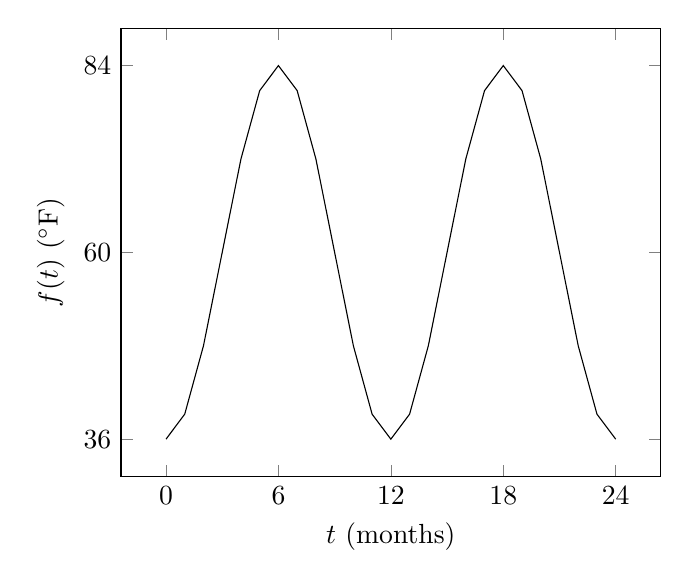
\begin{tikzpicture}
            \begin{axis}[
            xlabel=$t$ (months), ylabel=$f(t)$ ($^\circ$F),
            xtick={0, 6, 12, 18, 24}, ytick={36, 60, 84},
            ]
            \addplot[domain=0:24] {-24*cos(deg(x*pi/6))+60};
            \end{axis}
        \end{tikzpicture}
      \end{center}
    \end{solution}

  \item
    \begin{problem}[\stretch{0.5}]
      Find a formula for $f(t)$, the average temperature at time $t$ according to
      the model.
    \end{problem}

    \begin{solution}
      The amplitude is $\frac{84-36}{2}=\frac{48}{2}=24$.  The balance
      value is $60$ (half-way between $36$ and $84$).  The period is 12
      months.  We know that $t=0$ is the coldest date, so that means the
      sinusoid should look like the graph of $y=-\cos x$, since $-\cos x$
      is at a minimum at $x=0$. Thus, we get $f(t)=\boxed{-24
        \cos\left(\frac{\pi}{6}t\right)+60}.$
    \end{solution}

    \begin{grading}
      A common error was to use $\sin$ instead of $-\cos$, but the graph
      of $24 \sin \left( \frac{2 \pi}{12} t \right) + 60$ does not have a
      minimum at $t = 0$; instead, it is at the balance value when $t =
      0$: 
      \begin{center}
        \includegraphics[width=2in]{images/spring2012-mb-midterm1-1-incorrect}
      \end{center}
    \end{grading}

  \item
    \begin{problem}[\stretch{0.5}]
      According to the model, what was the average temperature on May 1, 2011?
      Simplify your answer.
    \end{problem}

    \begin{solution}
      May 1, 2011 corresponds to $t = 4$, so we are looking for $f(4)$.
      From our formula for $f$, we have
      \begin{align*}
        f(4)&=-24\cos\left(\frac{2\pi}{12} \cdot 4\right)+60 \\
        &= - 24 \cos \left( \frac{2 \pi}{3} \right) + 60 \\
        &= -24 \left( -\frac{1}{2} \right) + 60 \\
        &= \boxed{72}
      \end{align*}

      \checkmark\
        Quick consistency check: From the graph, we can see that, at $t =
        3$, the temperature should be at the balance value ($60^\circ)$
        and that the temperature at $t = 4$ should be higher than that.
    \end{solution}

    \pspace{\newpage}

      \item
    \begin{problem}[\stretch{1}]
      Using your model, determine the time(s) between $t=0$ and $t=24$ for which the average temperature was $50^\circ$F. Give exact answers. 
    \end{problem}

    \begin{solution}
      We can solve the following equation on the interval $[0, 24]$ to find the values of $t$.
      \begin{align*}
          -24\cos(\tfrac{\pi}{6}t)+60 &= 50 \\
          \cos(\tfrac{\pi}{6}t) &= \tfrac{5}{12}
          \intertext{
          We can make the substitution $\theta = \frac{\pi}{6}t$. Since we are looking for values of $t$ between $0$ and $24$, we should solve $\cos \theta = \tfrac{5}{12}$ for values of $\theta$ between $0$ and $4\pi$.
          }
          \cos \theta &= \arccos(\tfrac{5}{12}),\ 2\pi - \arccos(\tfrac{5}{12}),\
          2\pi + \arccos(\tfrac{5}{12}),\ 4\pi-\arccos(\tfrac{5}{12}) \\
          \intertext{Now we reverse the substitution and solve for $t$.}
          \tfrac{\pi}{6}t &= \arccos(\tfrac{5}{12}),\ 2\pi - \arccos(\tfrac{5}{12}),\
          2\pi + \arccos(\tfrac{5}{12}),\ 4\pi-\arccos(\tfrac{5}{12})  \\
          t &= \tfrac{6}{\pi}\arccos(\tfrac{5}{12}),\ 12- \tfrac{6}{\pi}\arccos(\tfrac{5}{12}),\ 12+\tfrac{6}{\pi}\arccos(\tfrac{5}{12}),\ 24-\tfrac{6}{\pi}\arccos(\tfrac{5}{12})
      \end{align*}
      We can check our answers against the graph to see if they make sense.

    \end{solution}

  
  \end{enumerate}
  
  % \item \label{estimate-height-of-tree} 

  %   \begin{problem}[\vfill\newpage]
  %     You are standing on flat ground trying to estimate the height of a
  %     tree. You first measure that the angle of elevation from the ground to
  %     the top of the tree is $\dfrac{\pi}{6}$. Then you move 100 feet closer
  %     to the tree and find that the angle of elevation is now
  %     $\dfrac{\pi}{4}$. How tall is the tree?  (Please simplify your
  %     answer.) 
  %   \end{problem}

  %   \begin{solution}
  %     Let $h$ be the height of the tree and $x$ be your distance from the
  %     tree after you've moved 100 feet closer.
  %     \begin{center}
  %       \includegraphics[width=2in]{images/estimate-height-of-tree}
  %     \end{center}
  %     From this diagram, we can see that $\displaystyle \tan \frac{\pi}{6}
  %     = \frac{h}{100 + x}$ and $\displaystyle \tan \frac{\pi}{4} =
  %     \frac{h}{x}$.  We'd like to use these facts to solve for $h$.  Let's
  %     start with the second equation:
  %     \begin{align*}
  %       \tan \frac{\pi}{4} &= \frac{h}{x} \\
  %       1 &= \frac{h}{x} \\
  %       x &= h
  %     \end{align*}
  %     Now, plugging the fact that $x = h$ into the first equation gives
  %     \begin{align*}
  %       \tan \frac{\pi}{6} &= \frac{h}{100 + h} \\
  %       \frac{1}{\sqrt{3}} &= \frac{h}{100 + h} \\
  %       \intertext{Cross-multiplying,}
  %       100 + h &= \sqrt{3} h \\
  %       100 &= \sqrt{3} h - h \\
  %       100 &= h (\sqrt{3} - 1) 
  %     \end{align*}
  %     So, $h = \boxed{\frac{100}{\sqrt{3} - 1}}$.       
  %   \end{solution}




\item \label{log-diff-curve-sketch-2} 

  In this problem, you'll look at $f(x) = 3x^{-2x}$ on $(0, \infty)$.

  \begin{enumerate}

  \item
    \begin{problem}[1in]
      Evaluate $f( \frac{1}{4})$.
    \end{problem}

    \begin{solution}
      \begin{align*}
        f (\tfrac{1}{4}) &= 3( \tfrac{1}{4}
        )^{-1/2} \\
        &= \frac{3}{\sqrt{1/4}} \\
        &= \frac{3}{1 / 2} \\
        &= \boxed{6}
      \end{align*}
    \end{solution}

  \item
    \begin{problem}[1in]
      Find all $x$-intercepts of $y=f(x)$ on $(0, \infty)$, or explain why
      there are none. 
    \end{problem}

    \begin{solution}
      We are looking for all values of $x$ such that $3x^{-2x} = 0$, or
      $x^{-2x} = 0$.  But since $x > 0$, there are \fbox{no such values}
      (a positive number raised to any power is always positive). 
    \end{solution}

  \item
    \begin{problem}[\vfill]
      Find $f'(x)$.
    \end{problem}

    \begin{solution}
      First, we can use the Constant Multiple rule: $f(x)$ is $3$ times
      $x^{-2x}$, so $f'(x)$ is 3 times the derivative of $x^{-2x}$.  To
      find the derivative of $x^{-2x}$, we'll use logarithmic
      differentiation because  both the base and the exponent depend on
      $x$.  Let's first give $x^{-2x}$ a new name, like
      $g(x)$:\footnote{When we do logarithmic differentiation, it's
        important to work with \emph{equations}, so we always want to
        start by giving a name to the thing we're differentiating.}
      \begin{align*}
        g(x) &= x^{-2x} \\
        \intertext{Take the natural log of both sides and simplify the right
          side:}
        \ln g(x) &= \ln \left( x^{-2x} \right) \\
        &= -2t \ln t 
        \intertext{Differentiate both sides with respect to $x$:}
        \frac{d}{dx} \left(\fcolorbox{red}{white}{$\displaystyle
            \ln\left(\fcolorbox{blue}{white}{$\displaystyle
                g\left(x\right)$}\right)$}\right) &=
        \frac{d}{dx} \left(\fcolorbox{purple}{white}{$\displaystyle
            -2$}\cdot x\cdot \ln x\right) \\
        \frac{1}{g(x)} g'(x) &=
        -2\cdot \frac{d}{dx} \left(\fcolorbox{green}{white}{$\displaystyle
            x$}\cdot \fcolorbox{green}{white}{$\displaystyle  \ln
            x$}\right) \\
        \frac{g'(x)}{g(x)} &= -2 \left(x\cdot \frac{1}{x}+ \ln x\right) \\
        &= -2 \left( 1 + \ln x \right) 
        \intertext{Solve for $g'(x)$:} %
        g'(x) &= g(x) \left[ -2 \left( 1 + \ln x \right) \right] \\
        &= -2 x^{-2x} \left( 1 + \ln x \right)
      \end{align*}
      Finally, remember that $f(x) = 3 g(x)$, so $f'(x) = 3 g'(x) =
      \boxed{-6 x^{-2x} \left( 1 + \ln x \right)}$. 
    \end{solution}

    \pspace{\newpage}

  \item
    \begin{problem}[\vfill]
      For what values of $x$ is $f(x)$ increasing?  Remember the domain is $(0, \infty)$.
    \end{problem}

    \begin{solution}
      \ideas{To answer this, let's make a sign chart for $f'$, since we
        know that the sign of $f'$ tells us whether $f$ is increasing or
        decreasing.}

      First, we'll find the critical points, where $f'(x) = 0$.
      \begin{align*}
        -6 x^{-2x} \left( 1 + \ln x \right) &= 0 \\
        \intertext{If a product is 0, one of the pieces of the product
          must be 0.  In this case, since we're only interested in where
          $x > 0$, $x^{-2x}$ will never be 0.  So, we must have:}
        1 + \ln x &= 0 \\
        \ln x &= -1 \\
        x &= e^{-1} = \frac{1}{e}
      \end{align*}
      Now, we test points.  It helps to notice that $x^{-2x}$ is always
      positive on $(-0, \infty)$, so we're really just testing the sign
      of $-6(1 + \ln x)$.  When $x = 1$, $-6 (1 + \ln x) = -6 < 0$; when
      $x = \frac{1}{e^2} = e^{-2}$, $-6(1 + \ln x) = -6 (1 - 2) > 0$.
      That gives us the following sign chart: 
      \begin{center}
        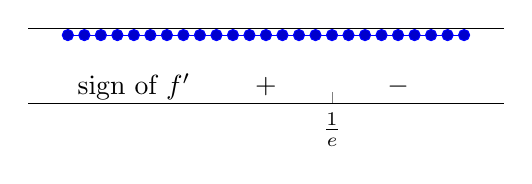
\begin{tikzpicture}
          \begin{axis}[axis y line=none, x axis line style={-}, xtick={0.367879}, xticklabels={$\frac{1}{e}$}, ymin=-2, height=1in, width=3in]
            \addplot+[domain=0.167879:0.467879]{0};
            \draw (axis cs: 0.167879, -1.5) node[right] {sign of $f'$};
            \draw (axis cs: 0.317879, -1.5) node{$+$};
            \draw (axis cs: 0.417879, -1.5) node{$-$};
          \end{axis}
        \end{tikzpicture}
      \end{center}
      So, $f$ is increasing on $\boxed{\left(0, \frac{1}{e} \right)}$.  
    \end{solution}

  \item
    \begin{problem}[0.5in]
      What is $\displaystyle \lim_{x \to \infty} f(x)$? 
    \end{problem}

    \begin{solution}
      If $x$ is large, then $x^{-2x}$ involves raising a very large number
      to a very negative number, so the result will be very close to 0.
      So, $\displaystyle \lim_{x \to \infty} f(x) = \boxed{0}$.     
    \end{solution}

  \item 

    $\displaystyle \lim_{x \to 0^+} f(x)$ is equal to one of the
    following.  Which one?\footnote{You are not expected to be able to
      evaluate $\displaystyle \lim_{x \to 0^+} 3x^{-2x}$.  Rather, you
      should be able to use what you've done so far in this problem to
      eliminate two of the three choices.}  No explanation is necessary. 
    \begin{multicols}{3}
      \begin{enumerate}[label=\protect\maybecircle{\Alph*.}]
      \plainitem $-1$
      \circleitem $3$
      \plainitem $9$
      \end{enumerate}
    \end{multicols}

    \begin{solution}
      Since we know that $f(x)$ has no $x$-intercepts and that $f \left(
        \frac{1}{4} \right) > 0$, there is no way that $\displaystyle
      \lim_{x \to 0^+} f(x)$ could be negative.\footnote{Technically, we
        are also using the fact that $f$ is continuous.}  So, we can
      eliminate choice A.

      In addition, since we know that $f(x)$ is increasing on $\left( 0,
        \frac{1}{e} \right)$, we know that $\displaystyle \lim_{x \to 0^+}
      f(x)$ must be lower than $f \left( \frac{1}{4} \right) = 6$.  This
      eliminates choice C, so choice B must be the correct one. 
    \end{solution}


  \item
    \begin{problem}[\vfill]
      Sketch $f(x)$ on $(0, \infty)$.  Your answer should reflect your
      work from the previous parts, but you need not show the concavity
      accurately.  Label the coordinates of any local extrema on your
      graph.
    \end{problem}

    \begin{solution}
      \begin{center}
        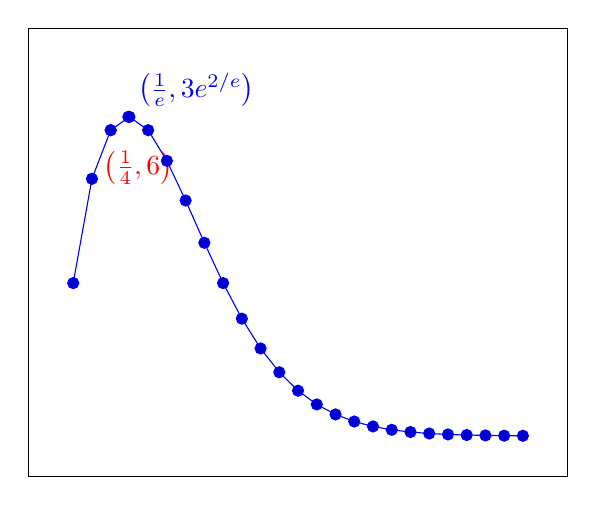
\begin{tikzpicture}
          \begin{axis}[xtick=\empty, ytick=\empty, ymax=8]
            \addplot+[domain=0:3] {3 * x^(-2*x)};
            \draw[red, fill=red] (axis cs: 0.25, 6) circle(2pt)
            node[below, xshift=1em, yshift=-4pt] {$\left( \frac{1}{4}, 6 
              \right)$};
            \draw[blue, fill=blue] (axis cs: 0.367879, 6.2612) circle(2pt)
            node[anchor=south west] 
            { $\left( \frac{1}{e}, 3 e^{2/e} \right)$};
          \end{axis}
        \end{tikzpicture}
      \end{center}
    \end{solution}

  \end{enumerate}

  \pspace{\newpage}

\item \label{spring2010-midterm2-7} 
  
  In each part, find the specified value, or explain why it does not
  exist.  Please show your work. 

  \begin{multicols}{2}
  \begin{enumerate}
  \item
    \begin{problem}
      $
      \sin\!\left(\arctan(\frac{-1}{\sqrt{3}})\right)$ 
    \end{problem}
    \pspace{1.5in}

    \begin{solution} 
      First we focus on the inside:
      $\arctan\left(\frac{-1}{\sqrt{3}}\right)$ is defined to be the angle
      in $\left( - \frac{\pi}{2}, \frac{\pi}{2} \right)$ whose tangent
      value is $\frac{-1}{\sqrt{3}}$.  The single such angle is
      $-\frac{\pi}{6}$, so $\arctan \left( - \frac{1}{\sqrt{3}} \right) =
      - \frac{\pi}{6}$.

      So, the question is asking us for $\sin \left( - \frac{\pi}{6}
      \right)$, which is $\boxed{- \frac{1}{2}}$. 
    \end{solution}

  \item
    \begin{problem}
      $
      \tan^{-1}\!\left(\tan(\frac{11\pi}{4})\right)$
    \end{problem}
    \pspace{1.5in}

    \begin{solution}
      We can evaluate $\tan \left( \frac{11 \pi}{4} \right) = -1$, so this
      is asking for $\arctan (-1)$, which is $\boxed{-\frac{\pi}{4}}$.
    \end{solution}

  \item
    \begin{problem}
      $\tan(\tan^{-1}(2))$
    \end{problem}
    \pspace{1.5in}
    
    \strut

    \begin{solution}
      Here, the inside is not a ``nice'' number that we know, so let's
      just give it a name: if we let $\theta = \tan^{-1} (2)$, then we are
      looking for $\tan \theta$.

      Let's think about what saying $\theta = \tan^{-1}(2)$ means.  By
      definition, this means that $\theta$ is the angle in $\left( -
        \frac{\pi}{2}, \frac{\pi}{2} \right)$ whose tangent value is 2.
      In other words, $\tan \theta = 2$.

      But we are looking for $\tan \theta$, and we've just seen that it is
      $\boxed{2}$. 
    \end{solution}

    \columnbreak

  \item
    \begin{problem}
      $\cos\!\left(\arcsin\left(\frac{5}{3}\right)\right)$
    \end{problem}
    \pspace{1.5in}

    \begin{solution}
      The domain of $\arcsin(x)$ is the same as the range of $\sin(x)$
      which is $[-1,1]$. Since $5/3>1$, $\arcsin\left(\frac{5}{3}\right)$
      does not exist, so $\cos \left( \arcsin \left( \frac{5}{3} \right)
      \right)$ \fbox{does not exist}.
    \end{solution}

  \item
    \begin{problem}
      $\sin\!\left(\arccos\left(- \frac{3}{5}\right)\right)$
    \end{problem}
    \pspace{1.5in} 

    \begin{solution}
      Here, the inside is not a ``nice'' number that we know, so let's
      just give it a name: if we let $\theta = \arccos \left( - \frac{3}{5}
      \right)$, then we are looking for $\sin \theta$.

      Let's think about what saying $\theta = \arccos \left( - \frac{3}{5}
      \right)$ means.  By definition, this means that $\theta$ is the
      angle in $[0, \pi]$ whose cosine is $- \frac{3}{5}$.  We can picture
      that as the following angle (with the reference triangle shown).
      \begin{center}
        
\includegraphics[width=1.75in]{Exam 1/Practice Exams/spring2010-midterm2-7e.pdf} 
      \end{center}
      We know that, in the reference triangle,
      $\dfrac{\text{adjacent}}{\text{hypotenuse}} = \dfrac{3}{5}$, so we've
      labeled the adjacent side $\dfrac{3}{5}$ and the hypotenuse
      $1$.\footnote{This is not the only option; you could also, for
        instance, label the adjacent side 3 and the hypotenuse 5.}
      Then, using the Pythagorean Theorem, we found that the opposite side
      (in red) must have length $\dfrac{4}{5}$.

      Now, we can see from the diagram that sine of this angle is $\boxed{
        \frac{4}{5}}$.
    \end{solution}

  \end{enumerate}
  \end{multicols}
  
  \item Find the derivative of $f(x)=(\arctan x)^x$.

  \begin{solution}
      \begin{align*}
          \ln(f(x)) &= \ln\!\left((\arctan x)^x\right) \\
          &= x\ln(\arctan x) \\
          \frac{f'(x)}{f(x)} &= \ln(\arctan x) + x\left(\frac{1}{\arctan x}\cdot \frac{1}{1+x^2}\right)\\
          &= \ln(\arctan x) + \frac{x}{(1+x^2)\arctan x}\\
          f'(x) &= (\arctan x)^x \left(\ln(\arctan x) + \frac{x}{(1+x^2)\arctan x}\right)
      \end{align*}
  \end{solution}
  \pspace{\vfill}
  \pspace{\newpage}

\item \label{spring2010-midterm1-5-modified}

  \label{spring2010-mb-midterm1-5-modified} 

  One morning, Eric is making coffee using a cone-shaped dripper like the
  one shown below.  Coffee drips from the bottom of the
  dripper into a cylindrical mug.

          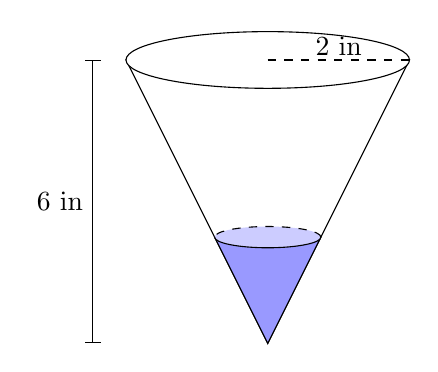
\begin{tikzpicture}[x=0.3cm, y=0.3cm]
          \def\R{6}
          \def\H{12}
          \def\r{2.25}
          \def\h{4.5}
          \def\aspect{5}
          \draw [fill=white] (-\R,\H) -- (\R,\H) -- (0,0) -- cycle;
          \draw [fill=white] (0, \H) circle [x radius=\R, y
          radius={\R/\aspect}];
          \draw [fill=blue!40!white,opacity=1] (-\r, \h) -- (\r, \h) --
          (0,0) -- cycle; 
          \draw [fill=blue!20!white,opacity=1, draw opacity=0] (0, \h) ellipse
          [x radius=\r, 
          y radius={\r/\aspect}];
          \draw (-\r, \h) arc [x radius=\r, y radius={\r/\aspect}, start
          angle=180, end angle=360];      
          \draw[dashed] (\r, \h) arc [x radius=\r, y radius={\r/\aspect},
          start angle=0, end angle=180];
          \draw[dashed] (0, \H) -- node[yshift=5pt]{2 in} (\R, \H);
          \draw[|-|, xshift=-12pt] (-\R, 0) -- node[left]{6 in} (-\R,
          \H);
        \end{tikzpicture} 

  Suppose Eric's dripper and mug each have radius 2 inches and height 6
  inches, and coffee drips at a constant rate of 5 in$^3$/min from the
  dripper into the mug.

  \begin{enumerate}
  \item \label{spring2010-mb-midterm1-5a}
    \begin{problem}[\newpage]
      How quickly is the height of coffee in the dripper decreasing when
      the height of coffee in the dripper is 1.5 in? 
    \end{problem}

    \begin{solution}
      \ideas{We're given a picture, but it's not exactly the picture we
        want; the given picture shows the filter and carafe, but we are
        interested in the amount of coffee in the filter.  So, let's start
        by drawing our generic picture, which applies at any time.}

      Here is a picture of the situation:
      \begin{center}
        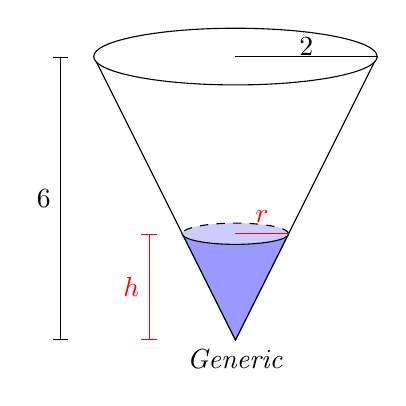
\begin{tikzpicture}[x=0.3cm, y=0.3cm]
          \def\R{6}
          \def\H{12}
          \def\r{2.25}
          \def\h{4.5}
          \def\aspect{5}
          \draw [fill=white] (-\R,\H) -- (\R,\H) -- (0,0) -- cycle;
          \draw [fill=white] (0, \H) circle [x radius=\R, y
          radius={\R/\aspect}];
          \draw [fill=blue!40!white,opacity=1] (-\r, \h) -- (\r, \h) --
          (0,0) -- cycle; 
          \draw [fill=blue!20!white,opacity=1, draw opacity=0] (0, \h) ellipse
          [x radius=\r, 
          y radius={\r/\aspect}];
          \draw (-\r, \h) arc [x radius=\r, y radius={\r/\aspect}, start
          angle=180, end angle=360];      
          \draw[dashed] (\r, \h) arc [x radius=\r, y radius={\r/\aspect},
          start angle=0, end angle=180];
          \draw (0, \H) -- node[above, inner sep=0.1pt]{2} (\R, \H);
          \draw[|-|, xshift=-12pt] (-\R, 0) -- node[left]{6} (-\R,
          \H);
          \draw[red] (0, \h) -- node[above, inner sep=0, yshift=4pt]{$r$} (\r, \h);
          \draw[red, |-|, xshift=-12pt] (-\r, 0) -- node[left]{$h$} (-\r,
          \h);
          \draw (0, 0) node[below, font=\normalsize]{\emph{Generic}};
        \end{tikzpicture} \hspace{0.5in}
        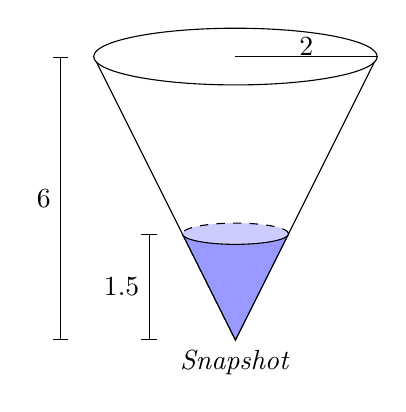
\begin{tikzpicture}[x=0.3cm, y=0.3cm]
          \def\R{6}
          \def\H{12}
          \def\r{2.25}
          \def\h{4.5}
          \def\aspect{5}
          \draw [fill=white] (-\R,\H) -- (\R,\H) -- (0,0) -- cycle;
          \draw [fill=white] (0, \H) circle [x radius=\R, y
          radius={\R/\aspect}];
          \draw [fill=blue!40!white,opacity=1] (-\r, \h) -- (\r, \h) --
          (0,0) -- cycle; 
          \draw [fill=blue!20!white,opacity=1, draw opacity=0] (0, \h) ellipse
          [x radius=\r, 
          y radius={\r/\aspect}];
          \draw (-\r, \h) arc [x radius=\r, y radius={\r/\aspect}, start
          angle=180, end angle=360];      
          \draw[dashed] (\r, \h) arc [x radius=\r, y radius={\r/\aspect},
          start angle=0, end angle=180];
          \draw (0, \H) -- node[above, inner sep=0.1pt]{2} (\R, \H);
          \draw[|-|, xshift=-12pt] (-\R, 0) -- node[left]{6} (-\R,
          \H);
          \draw[|-|, xshift=-12pt] (-\r, 0) -- node[left]{1.5} (-\r,
          \h);
          \draw (0, 0) node[below, font=\normalsize]{\emph{Snapshot}};
        \end{tikzpicture} 
      \end{center}
      The variables in red ($r$, the radius of the liquid, and $h$, the
      height of the liquid) are changing, while the values in blue are
      constant.  We'll also write $V$ for volume. 

      \ideas{Next, we figure out what we know and what we want to know.}

      \highlight{
        \textbf{What we know:} $\dfrac{dV}{dt} = -5$ (this is negative
        because the volume of coffee in the filter is decreasing: coffee is
        leaving the filter)

        \textbf{What we want to know:} $\dfrac{dh}{dt}$
      }

      \ideas{Now, we try to relate variables.  In this case, since the rate
        we know about is $\frac{d\bm{V}}{dt}$ and the rate we want to know
        is $\frac{d\bm{h}}{dt}$, we try to relate $V$ and $h$. }

      We know that $V = \dfrac{1}{3} \pi r^2 h$.

      \ideas{This is a good start, but we'd ideally like to relate just $V$
        and $h$ without $r$ mucking things up.  So, let's see if we can
        write $r$ in terms of $V$ and $h$.  In this case, we can do that
        using similar triangles.}

      Let's focus on the blue triangle shown in the following picture:
      \begin{center}
        \begin{center}
          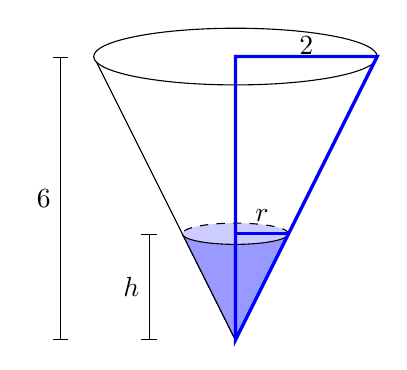
\begin{tikzpicture}[x=0.3cm, y=0.3cm]
            \def\R{6}
            \def\H{12}
            \def\r{2.25}
            \def\h{4.5}
            \def\aspect{5}
            \draw [fill=white] (-\R,\H) -- (\R,\H) -- (0,0) -- cycle;
            \draw [fill=white] (0, \H) circle [x radius=\R, y
            radius={\R/\aspect}];
            \draw [fill=blue!40!white,opacity=1] (-\r, \h) -- (\r, \h) --
            (0,0) -- cycle; 
            \draw [fill=blue!20!white,opacity=1, draw opacity=0] (0, \h) ellipse
            [x radius=\r, 
            y radius={\r/\aspect}];
            \draw (-\r, \h) arc [x radius=\r, y radius={\r/\aspect}, start
            angle=180, end angle=360];      
            \draw[dashed] (\r, \h) arc [x radius=\r, y radius={\r/\aspect},
            start angle=0, end angle=180];
            \draw[blue, very thick] (0, 0) -- (0, \H) --
            node[above, inner sep=0.1pt, black]{2}
            (\R, \H) -- cycle;      
            \draw[blue, very thick] (0, \h) -- node[above, inner sep=0, 
            black, yshift=4pt]{$r$} (\r, \h); 
            \draw[|-|, xshift=-12pt] (-\R, 0) -- node[left]{6} (-\R,
            \H);
            \draw[|-|, xshift=-12pt] (-\r, 0) -- node[left]{$h$} (-\r,
            \h);
          \end{tikzpicture}
        \end{center}    
      \end{center}
      We can see that it is similar to the smaller triangle inside of it, so
      \begin{align*}
        \frac{r}{h} &= \frac{2}{6} \\
        r &= \frac{h}{3}
      \end{align*}
      We can plug this in to our equation $V = \dfrac{1}{3} \pi r^2 h$ to
      get: 

      \highlight{\textbf{Equation relating our variables:} $\displaystyle V
        = \frac{1}{3} \pi \left( \frac{h}{3} \right)^2 h = \frac{1}{27} \pi
        h^3$}  

      \ideas{Once we have our relating equation, we differentiate it.  Since
        we are looking for $\frac{dh}{d\bm{t}}$, we should differentiate it
        with respect to $t$.}
      \[ \frac{dV}{dt} = \frac{1}{9} \pi h^2 \frac{dh}{dt}\]
      \ideas{Finally, we can plug in the values at the time we care about:}
      \begin{align*}
        -5 &= \frac{1}{9} \pi \left( \frac{3}{2} \right)^2
        \frac{dh}{dt} \\
        &= \frac{1}{4} \pi \frac{dh}{dt} \\
        - \frac{20}{\pi} &= \frac{dh}{dt}
      \end{align*}
      That is, the height of coffee in the filter is \fbox{decreasing at an
        instantaneous rate of $\dfrac{20}{\pi}$ in$^3$/min}.
    \end{solution}

  \item
    \begin{problem}[\vfill]
      As time passes, does the height of the coffee in the dripper
      decrease more quickly, more slowly, or at a constant rate?  Please
      explain by referring to a formula.  (Does your answer make sense
      intuitively?)  
    \end{problem}

    \begin{solution}
      In \ref{spring2010-mb-midterm1-5a}, we found that $\displaystyle
      \frac{dV}{dt} = \frac{1}{9} \pi h^2 \frac{dh}{dt}$, so
      $\displaystyle \frac{dh}{dt} = \frac{9}{\pi h^2} \frac{dV}{dt}$.  We
      know that $\dfrac{dV}{dt} = -5$ (always, because the coffee drips at
      a constant rate), so $\displaystyle \frac{dh}{dt} = - \frac{45}{\pi
        h^2}$.  As time goes on, $h$ (the height of coffee in the dripper)
      decreases, which means that $-\frac{45}{\pi h^2}$ becomes more and
      more negative.  \fbox{So, as the height of the coffee in the dripper
        decreases, it will do so at a faster and faster rate.}
    \end{solution}

  \item
    \begin{problem}[\vfill]
      As time passes, does the height of the coffee in the mug increase
      more quickly, more slowly, or at a constant rate?  Please explain
      briefly.  (A ``common sense'' answer is sufficient.)
    \end{problem}

    \begin{solution}      
      The height of coffee in the mug \fbox{increases at a constant
        rate}.  This may be intuitively obvious, but we can also justify
      it mathematically.  If $V$ is the volume of coffee in the mug and
      $h$ is the height, we know that $V = \pi \cdot 2^2 \cdot h = 4 \pi
      h$ (the coffee forms a cylinder of radius 2).  Differentiating with
      respect to $t$ gives
      \[ \frac{dV}{dt} = 4 \pi \frac{dh}{dt}.\] If coffee is dripping at a
      constant rate of 5 in$^3$/min into the mug, then $\dfrac{dV}{dt} =
      5$ (positive because the volume of coffee in the mug is increasing),
      so $\dfrac{dh}{dt} = \dfrac{5}{4 \pi}$, which is clearly constant.

      (The key point is that the radius of the coffee in the cylindrical
      mug is the same at any height, unlike in the conical dripper.)
    \end{solution}

  \item
    \begin{problem}[\vfill\newpage]
      Let $D$ be the volume of coffee in the dripper and $M$ be the volume
      of coffee in the mug.  What is the sign of $\displaystyle
      \frac{dD}{dM}?$ Please explain briefly. 
    \end{problem}

    \begin{solution}
      One way to think about this is: If we graphed $D$ as a function of
      $M$, would we have an increasing or decreasing function?  We know
      that as $M$ increases (more coffee in the mug), $D$ decreases (less
      coffee in the dripper), so the graph described would be decreasing.
      That means that $\dfrac{dD}{dM}$ must be \fbox{negative}.
    \end{solution}

  \end{enumerate}  


\item
    \label{spring2007-midterm2-5}

    Match each graph with its equation.  Write your answers in the blanks
    below each graph.  No explanation is needed. 

    \begin{tabular}{c c c}
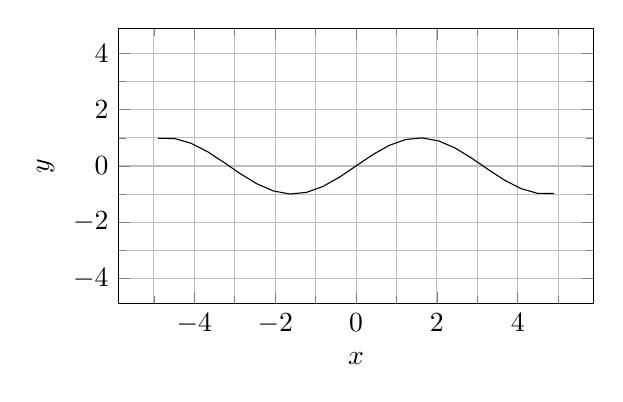
\begin{tikzpicture}
    \begin{axis}[xlabel=$x$, ylabel=$y$,ymin=-4.9, ymax=4.9, xtick distance=2, ytick distance=2, minor tick num=1, width=3in, height=2in, grid=both,]
        \addplot[domain=-4.9:4.9] {sin(deg(x))};
    \end{axis}
\end{tikzpicture}
      & \hspace{0.25in} & 
      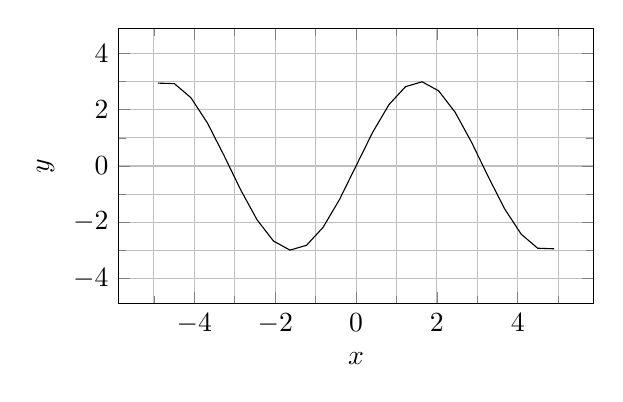
\begin{tikzpicture}
    \begin{axis}[xlabel=$x$, ylabel=$y$,ymin=-4.9, ymax=4.9, xtick distance=2, ytick distance=2, minor tick num=1, width=3in, height=2in, grid=both,]
        \addplot[domain=-4.9:4.9] {3*sin(deg(x))};
    \end{axis}
\end{tikzpicture}
      \\ \\
      Function: \fitb{0.5in}{C} && Function: \fitb{0.5in}{E} \\ \\ \\
      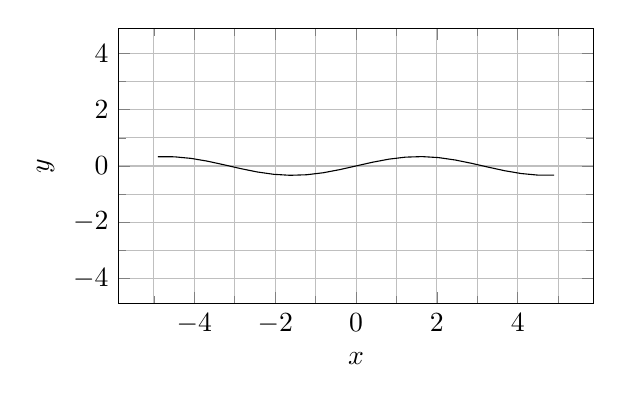
\begin{tikzpicture}
    \begin{axis}[xlabel=$x$, ylabel=$y$,ymin=-4.9, ymax=4.9, xtick distance=2, ytick distance=2, minor tick num=1, width=3in, height=2in, grid=both,]
        \addplot[domain=-4.9:4.9] {(1/3)*sin(deg(x))};
    \end{axis}
\end{tikzpicture}
      & &
      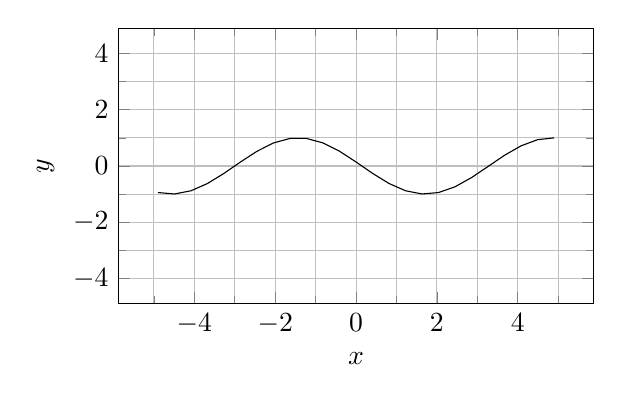
\begin{tikzpicture}
    \begin{axis}[xlabel=$x$, ylabel=$y$,ymin=-4.9, ymax=4.9, xtick distance=2, ytick distance=2, minor tick num=1, width=3in, height=2in, grid=both,]
        \addplot[domain=-4.9:4.9] {sin(deg(x+3))};
    \end{axis}
\end{tikzpicture}
      \\ \\
      Function: \fitb{0.5in}{F} && Function: \fitb{0.5in}{G} \\ \\ \\    
      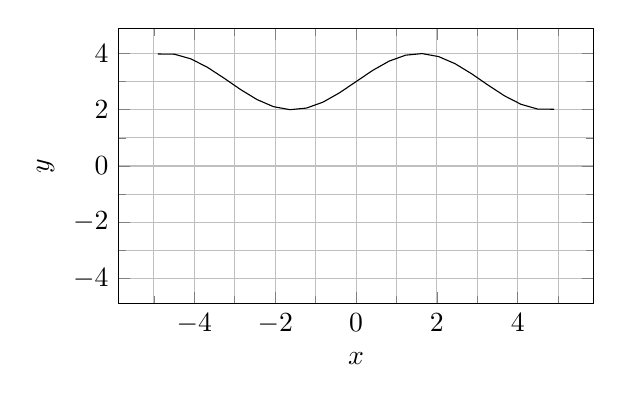
\begin{tikzpicture}
    \begin{axis}[xlabel=$x$, ylabel=$y$,ymin=-4.9, ymax=4.9, xtick distance=2, ytick distance=2, minor tick num=1, width=3in, height=2in, grid=both,]
        \addplot[domain=-4.9:4.9] {sin(deg(x))+3};
    \end{axis}
\end{tikzpicture}
      & & 
      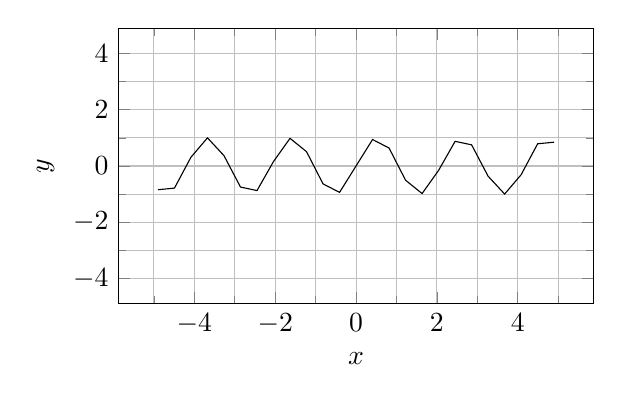
\begin{tikzpicture}
    \begin{axis}[xlabel=$x$, ylabel=$y$,ymin=-4.9, ymax=4.9, xtick distance=2, ytick distance=2, minor tick num=1, width=3in, height=2in, grid=both,]
        \addplot[domain=-4.9:4.9] {sin(deg(3*x))};
    \end{axis}
\end{tikzpicture}
      \\ \\
      Function: \fitb{0.5in}{A} && Function: \fitb{0.5in}{B} 
    \end{tabular}

    \bigskip

    Choices:
    \begin{multicols}{4}
      \begin{enumerate}[label=(\Alph*)]
      \item $y=\sin(x) + 3$
      \item $y=  \sin(3x)$
      \item $y=\sin(x)$
      \item $y=  \sin(\frac{x}{3})$
      \item $y=3\sin(x)$
      \item $y=  \frac{\sin(x)}{3}$
      \item $y=\sin(x + 3)$ 
      \item $y=  \sin(x)-3$
      \end{enumerate}
    \end{multicols}

    \pspace{\newpage}

%   \item \label{trig-graph-pick-1} 

%     Now, we'll look at $f(x) = x \sin (\pi x^2)$.

%     \begin{enumerate}
%     \item \label{trig-graph-pick-1-symmetry}
%       \begin{problem}[1.25in]
%         Is $f(x)$ an even function, an odd function, or neither?  Justify
%         your answer.  
%       \end{problem}

%       \begin{solution}
%         To test this, we should look at $f(-x)$.
%         \begin{align*}
%           f(-x) &= (-x) \sin [\pi (-x)^2] \\
%           &= - x \sin (\pi x^2) \\
%           &= - f(x)
%         \end{align*}
%         So, $f$ is \fbox{an odd function}. 
%       \end{solution}

%     \item \label{trig-graph-pick-1-intercepts}
%       \begin{problem}[\vfill]
%         Find all $x$-intercepts of $f(x)$. 
%       \end{problem}

%       \begin{solution}
%         We want to solve $f(x) = 0$:
%         \[ x \sin \left( \pi x^2 \right) = 0\]
%         In order for a product to be 0, one of the factors
%         being multiplied must be 0:
%         \[ x = 0 \text{ or } \sin \left( \pi x^2 \right) = 0 \]
%         Let's work on the latter equation.  First, let's substitute $u =
%         \pi x^2$ to make it look simpler.  Then, we are solving
%         \[ \sin u = 0.\]
%         We know that the roots of sine occur at all integer multiples of
%         $\pi$, i.e.
%         \[ u = 0, \pm \pi, \pm 2 \pi, \pm 3 \pi, \ldots \text{(or,
%           more succinctly, $u = n \pi$ where $n$ is any integer)}\]
%         Now, since $u = \pi x^2$, this says that
%         \begin{alignat*}{3}
%           \pi x^2 &= 0, \pm \pi, \pm 2 \pi, \pm 3 \pi, \ldots & &= n \pi
%           \text{ where $n$ is any integer} \\
%           x^2 &= 0, \pm 1, \pm 2, \pm 3, \ldots & & = n \text{ where $n$
%             is any integer} \\
%           x &= 0, \pm 1, \pm \sqrt{2}, \pm \sqrt{3}, \ldots & &= \pm
%           \sqrt{n} \text{ where $n$ is any non-negative integer}
%         \end{alignat*}
%         So, the $x$-intercepts of $f(x)$ are $\boxed{0, \pm 1, \pm
%           \sqrt{2}, \pm \sqrt{3}, \ldots}$, which can also be written as      
%         \begin{center}
%           \fbox{$\pm \sqrt{n}$ where $n$ is any non-negative integer}. 
%         \end{center}        
%       \end{solution}

%     \item
%       Which of the following is the graph of $f(x)$? \fitb{0.5in}{C}  (No
%       explanation is necessary.)

%       \begin{multicols}{2}
%         \begin{enumerate}[label=\Alph*.]
%         \item
%           \raisebox{2ex-\height}{\begin{tikzpicture}
%     \begin{axis}[ymin=-4.1, ymax=4.1, xtick distance=2, ytick distance=2, minor tick num=1, width=2in, height=2in, grid=both, axis equal image, samples=200]
%         \addplot[domain=-4.1:4.1] {abs(x)*cos(deg(3*pi/(2*x)))};
%     \end{axis}
% \end{tikzpicture}}

%         \item
%           \raisebox{2ex-\height}{\begin{tikzpicture}
%     \begin{axis}[ymin=-4.1, ymax=4.1, xtick distance=2, ytick distance=2, minor tick num=1, width=2in, height=2in, grid=both, axis equal image, samples=200]
%         \addplot[domain=-4.1:4.1] {(4-0.75*abs(x))*sin(deg(pi*x^2))};
%     \end{axis}
% \end{tikzpicture}}

%         \item
%           \raisebox{2ex-\height}{\includegraphics[width=1.75in]{images/trig-graph-pick-1-choice3}}

%         \item
%           \raisebox{2ex-\height}{\includegraphics[width=1.75in]{images/trig-graph-pick-1-choice4}}

%         \end{enumerate}
%       \end{multicols}

      % \pspace{\newpage}

      % \begin{solution}
      %   In \ref{trig-graph-pick-1-symmetry}, we found that $f$ is odd.  Of
      %   the choices, only C and D show odd functions.  In
      %   \ref{trig-graph-pick-1-intercepts}, we found that that the
      %   $x$-intercepts of $f(x)$ are $0, \pm 1, \pm \sqrt{2}, \ldots$.  In
      %   particular, the $x$-intercepts are not evenly spaced, so this must
      %   be graph C.\footnote{Another way to see that graph D is incorrect
      %     is to notice that the smallest $x$-intercept of $f$ greater than
      %     0 is 1.}
      % \end{solution}

    % \end{enumerate}

\item 
  \label{spring2012-mb-midterm1-implicit-differentiation}

  The graph shown below is determined by the equation $x^4=5x^2-(x^2 -
  y)^2$.

  \begin{enumerate}
  \item
    \begin{problem}
      The graph intersects the $x$-axis at three points.  What are these
      points?
    \end{problem}

    
\includegraphics[height=1.75in]{assessments/Exam 1/Practice Exams/spring2012-mb-midterm1-implicit-differentiation.pdf} 

    \begin{solution}
      \ideas{The curve is defined by $x^4 = 5x^2 - (x^2 - y)^2$, and we
        want the intersection of this curve with $y = 0$.}

      If we plug $y = 0$ into the equation $x^4 = 5x^2 - (x^2 - y)^2$, we
      get
      \begin{align*}
        x^4 &= 5x^2 - (x^2)^2 \\
        x^4 &= 5x^2 - x^4 \\
        \intertext{Moving everything to one side,}
        2x^4 - 5x^2 &= 0 \\
        2x^2 \left(x^2 - \frac{5}{2} \right) &= 0
      \end{align*}
      A product is 0 if one of the pieces being multiplied is
      0, so either $x = 0$ or $x^2 = \frac{5}{2}$.  So, the three points
      where the graph intersects the $x$-axis are $\boxed{\left( - \sqrt{
            \frac{5}{2}}, 0 \right), (0, 0), \left( \sqrt{ \frac{5}{2}}, 0
        \right)}$. 
    \end{solution}

  \item
    \begin{problem}
      $(1, 3)$ is a point on this curve.  On the graph above, mark the
      rough location of $(1, 3)$ with a dot.
    \end{problem}

    \begin{solution}
      The right-most $x$-intercept is at $x = \sqrt{\frac{5}{2}} =
      \sqrt{2.5} > 1$, so $(1, 3)$ is to the left of that.  So, a
      reasonable estimate is the point shown here:
      \begin{center}
        
\includegraphics[height=1.75in]{assessments/Exam 1/Practice Exams/spring2012-mb-midterm1-implicit-differentiation-point.pdf}        
      \end{center}
    \end{solution}

  \item
    \begin{problem}[\vfill]
      Find the equation of the line tangent to the curve at $(1, 3)$.
    \end{problem}

    \begin{problemonly}
      \textbf{Your answer}: The equation of the tangent line is
      \fitb{2in}{} 
    \end{problemonly}

    \begin{solution}      
      \ideas{The slope of the tangent line is the value of the derivative
        $\dfrac{dy}{dx}$ at $(1, 3)$.  Since we have an equation that
        relates $x$ and $y$ but that doesn't say ``$y = $ something''
        directly, we'll use implicit differentiation to find this
        derivative.}

      We start with the equation of the curve:
      \begin{align*}
        x^4 &= 5x^2 - (x^2 - y)^2 \\
        \intertext{Differentiate both sides with respect to $x$:}
        4x^3 &= 10 x - 2 (x^2 - y) \left( 2x - \frac{dy}{dx} \right) \\
        \intertext{Plug in the point $(1, 3)$ and solve for
          $\frac{dy}{dx}$:} 
        4 (1)^3 &= 10 (1) - 2 (1^2 - 3) \left( 2 \cdot 1 - \frac{dy}{dx}
        \right) \\
        4 &= 10 + 4 \left( 2 - \frac{dy}{dx} \right) \\
        -6 &= 4 \left( 2 - \frac{dy}{dx} \right) \\
        - \frac{3}{2} &= 2 - \frac{dy}{dx} \\
        \frac{dy}{dx} &= 2 + \frac{3}{2} \\
        &= \frac{7}{2}
      \end{align*}
      So, the slope of the tangent line is $\frac{7}{2}$.  (Notice that
      this is positive, which agrees with our picture.)  Since $(1, 3)$ is
      a point on the line, an equation for the tangent line is $\boxed{y -
        3 = \frac{7}{2} (x - 1)}$.
    \end{solution}

  \end{enumerate}

  \pspace{\newpage}

  \continueproblem{\emph{Continued from previous page}}

  \begin{enumerate}[resume]
  \item
    \begin{enumerate}
    \item \label{spring2012-mb-midterm1-implicit-differentiation-linear-approx} 
      \begin{problem}[\vfill]
        Imagine that a bug is crawling along this curve.  He has just
        passed through $(1, 3)$, and his $x$-coordinate is now $0.9$.  Use
        linear approximation to estimate his $y$-coordinate.
      \end{problem}      

      \begin{problemonly}
        \textbf{Your answer}: The bug's approximate $y$-coordinate is
        \fitb{2in}{}
      \end{problemonly}

      \begin{solution}
        Near $(1, 3)$, the line $y - 3 = \frac{7}{2} (x - 1)$ should be
        very close to the graph of the actual curve $x^4 = 5x^2 - (x^2 -
        y)^2$.  So, the point on the \emph{line} with $x$-coordinate $0.9$
        should be a good approximation for the point on the \emph{curve}
        with $x = 0.9$.  The line can be rewritten as $y = 3 + \frac{7}{2}
        (x - 1)$, and if we plug in $x = 0.9$, we get $y = 3 + \frac{7}{2}
        (0.9 - 1) = 3 + 3.5 (-0.1) = 3 - 0.35 = \boxed{2.65}$. 
      \end{solution}

    \item
      \begin{problem}[\vfill\newpage]
        Does your answer to the last part
        seem reasonable given the picture?  Explain briefly.
      \end{problem}

      \begin{solution}
        Yes, if the bug's $x$-coordinate is a little less than 1, then
        he's a little bit to the left of the red point $(1, 3)$, which
        means that his $y$-coordinate should be a little bit smaller than
        3. 
      \end{solution}

    \end{enumerate}

  \end{enumerate}

  \end{enumerate}



\end{document}